\documentclass{article}

\date{13 décembre 2023}
\usepackage[nb-sem=11, auteurs={Kylian Boyet, Hugo Vangilluwen, Jérémie Menard, George Ober}]{../kholles}

\begin{document}
\maketitle

\begin{question_kholle}{Convergence d'une suite si ses sous-suites paires et impaires convergent}
  Soit $(a_{n})_{n \in \N}$ telle que $(a_{2n})_{n \in \N}$ et $(a_{2n+1})_{n \in \N}$ convergent vers la même limite $\ell$.
  Montrons que $a$ converge vers $\ell$.
  
  Soit $\varepsilon>0$. On veut construire un $N \in \N$ tel que $\forall n \geqslant N, \lvert a_{n} - \ell \rvert \leqslant \varepsilon$
  
  Appliquons la définition de la limite de $(a_{2n})_{n \in \N}$ et $(a_{2n+1})_{n \in \N}$
  
  \begin{align*}
    \exists N_{1} \in \N : \forall n \geqslant N_{1}, \lvert a_{2n} - \ell\rvert  \leqslant \varepsilon \\
    \exists N_{2} \in \N : \forall n \geqslant N_{2}, \lvert a_{2n+1} - \ell  \rvert \leqslant \varepsilon
  \end{align*}
  \begin{figure}[H]
    
    \centering
    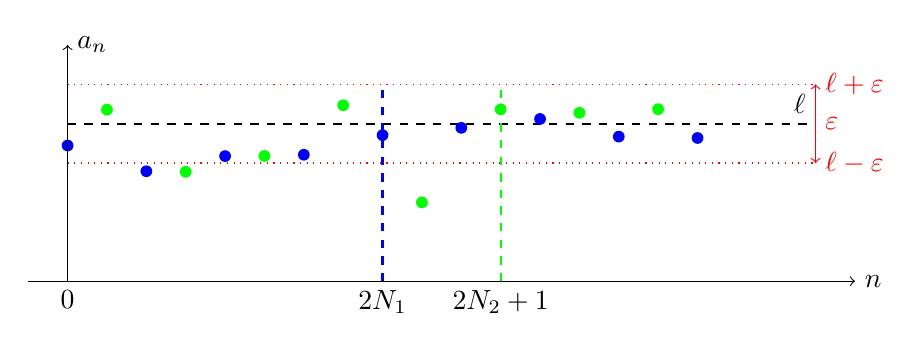
\begin{tikzpicture}
      \draw[thick, dashed] (0.5,2) -- (10,2) node[above left] {$\ell$};
      
      \draw[dotted, red] (0.5,2.5) -- (10,2.5) node[right] {$\ell + \varepsilon$};
      \draw[dotted, red] (0.5,1.5) -- (10,1.5) node[right] {$\ell - \varepsilon$};
      
      \foreach \x in {0.5, 1.5, 2.5, 3.5} {
      \node[circle, fill=blue, inner sep=1.5pt] at (\x, {1 + 0.8*rnd}) {}; % Odd terms
      }
      \foreach \x in {1, 2, 3, 4} {
      \node[circle, fill=green, inner sep=1.5pt] at (\x, {1 + 1.8*rnd}) {}; % Even terms
      }
      
      \node[circle, fill=green, inner sep=1.5pt] at (5, 1) {};
      
      \node[below] at (4.5,0) {$2N_1$};
      \draw[thick, dashed, blue] (4.5, 0) -- (4.5, 2.5) {};
      
      \node[below] at (6,0) {$2N_2 + 1$};
      \draw[thick, dashed, green] (6, 0) -- (6, 2.5) {};
      
      \foreach \x in {4.5, 5.5, 6.5, 7.5, 8.5} {
      \node[circle, fill=blue, inner sep=1.5pt] at (\x, {1.8 + 0.4*rnd}) {};
      }
      
      \foreach \x in { 6, 7, 8} {
      \node[circle, fill=green, inner sep=1.5pt] at (\x, {1.8 + 0.4*rnd}) {};
      }
      
      \draw[->] (0,0) -- (10.5,0) node[right] {$n$};
      \node[below] at (0.5,0) {$0$};
      
      \draw[->] (0.5,0) -- (0.5, 3) node[right] {$a_n$};
      
      \draw[<->, red] (10,2.5) -- (10,1.5);
      \node[right, red] at (10,2) {$\varepsilon$};
      
    \end{tikzpicture}
    \caption{Les termes pairs et impairs sont contenus dans un voisinnage de $\ell$ après certains rangs}
  \end{figure}
  
  Posons $N = \max(2N_{1}, 2N_{2}+1)$ et vérifions que ce rang convient.
  Soit $n \in \N$ tel que $n \geqslant N$. 
  \begin{itemize}[label=$\star$]
    \item Si $n$ est pair, $\exists p \in \N :$ $n = 2p$
$$
    n\geqslant N \geqslant 2N_{1} \implies 2p \geqslant 2N_{1} \implies p \geqslant N_{1}
$$
    Donc d'après la définition de la convergence de $(a_{2n})_{n \in \N}$, on a
$$
    \lvert a_{2p} - \ell \rvert  \leqslant \varepsilon \implies \lvert a_{n} - \ell  \rvert  \leqslant \varepsilon
$$
    
    \item Si $n$ est impair, $\exists p \in \N : n = 2p +1$
$$
    n \geqslant N \geqslant 2N_{2}+1 +\implies 2p+1 \geqslant 2N_{2} + 1 \implies p \geqslant N_{2}
$$
    Donc d'après la définition de la convergence de $(a_{2n+1})_{n \in \N}$, on a 
$$
    \lvert a_{2p+1} - \ell\rvert  \leqslant \varepsilon \implies \lvert a_{n} - \ell \rvert \leqslant \varepsilon
$$
  \end{itemize}
  Donc $\lvert a_{n} - \ell  \rvert\leqslant \varepsilon$
  Donc $a$ tend vers $\ell$.
  
\end{question_kholle}
\textbf{Remarque} Si les deux suites ne convergent pas vers la même limite, comme pour $((-1)^{n})_{n \in \N}$, la suite n'admet pas de limite.

\begin{question_kholle}
  [Soient $(A,B) \in (\mathcal{P}(\R) \setminus \{\varnothing\})^{2}$. Montrons que :
  \\
  $$A \text{ est dense dans } B \iff \left\{ \begin{array}{l}
    A \subset B \\
    \forall b \in B, \exists(a_{n}) \in A^{\N} : (a_{n}) \text{ converge vers }b
  \end{array}\right. $$
  ]
  {Caractérisation séquentielle de la densité.}
  
  Sens indirect : supposons $A \subset B$ et $\forall b \in B, \exists(a_{n}) \in A^{\N} : (a_{n}) \text{ converge vers }b$ :\\
  \begin{itemize}
    \item[$\star$] $A \subset B$ par hypothèse.
    \item[$\star$] Montrons que $\forall b \in B, \forall \varepsilon \in \R^{*}_{+}, \exists a \in A : |b - a| < \varepsilon$ (on utilise la caractérisation de la densité avec les $\varepsilon$) \\
    Soient $b \in B$ et $\varepsilon \in \R^{*}_{+}$ fixés quelconques : \\
    Par hypothèse appliquée pour $b \leftarrow b$ : $\exists(a_{n}) \in A^{\N} : a_{n} \underset{n \to +\infty}{\longrightarrow}b$ \\
    Appliquons la définition de la convergence de $(a_{n})$ vers $b$ pour $\varepsilon \leftarrow \frac{\varepsilon}{2}$ : \\
    $$\exists N \in \N : \forall n \in \N, n \geqslant N \Rightarrow |a_{n} - b| \leqslant \frac{\varepsilon}{2}$$
    Fixons un tel N : \\
    En particulier, $a_{N} \in A$ et $|a_{N} - b| \leqslant \frac{\varepsilon}{2} \leqslant \varepsilon$ \\
    Donc $A$ est dense dans $B$.
  \end{itemize}
  
  Sens direct : supposons $A$ dense dans $B$ : \\
  \begin{itemize}
    \item[$\star$] Par définition, $A \subset B$
    \item[$\star$] Soit $b \in B$ fixé quelconque. \\
    Soit $n \in \N$ fixé quelconque :  \\
    Appliquons la caractérisation de la densité par les $\varepsilon$ pour $\varepsilon \leftarrow \frac{1}{2^{n}}$ (autorisé car $\frac{1}{2^{n}} > 0$), et $b \leftarrow b$ :
    $$\exists a \in A : |a - b| \leqslant \frac{1}{2^{n}}$$
    Notons $a_{n}$ un tel élément. Nous venons de construire $(a_{n})_{n \in \N} \in A^{\N}$ vérifiant : \\
    $\forall n \in \N, |a_n - b| \leqslant \frac{1}{2^{n}}$ \\
    Or : $\underset{n \to +\infty}{\lim} \frac{1}{2^{n}} = 0$ \\
    Ainsi, d'après le théorème sans nom, $(a_{n})_{n \in \N}$ converge vers $b$.
  \end{itemize}
\end{question_kholle}

\begin{question_kholle}
  [Soit $u \in \R^\N$ une suite monotone :
  {\begin{enumerate}
    \item Si $u$ est croissante
    \begin{enumerate}[label=($\roman*$)]
      \item Soit $u$ est majorée, et dans ce cas, $\lim u = \sup\{ u_k | k \in \N \}$
      \item Soit $u$ n'est pas bornée, et dans ce cas, $u$ diverge vers $+\infty$.
    \end{enumerate}
    \item Si $u$ est décroissante :
    \begin{enumerate}[label=($\roman*$) Soit, leftmargin=4em]
      \item $u$ est minorée, et dans ce cas, $\lim u = \inf\{ u_k | k \in \N \}$
      \item $u$ n'est pas bornée, et dans ce cas, $u$ diverge vers $-\infty$.
    \end{enumerate}
  \end{enumerate} }]
  {Théorème de la convergence monotone}
  
  Soit $u \in \R^\N$ monotone fq.
  
  \begin{enumerate}
    \item Supposons que $u$ est croissante.
    \begin{enumerate}[label=($\roman*$)]
      \item Supposons que $u$ est majorée. \\
      Alors $\exists M \in \R : \forall n \in \N, u_n \leqslant M$. Fixons un tel M. \\
      $\Omega = \{ u_k | k \in \N \}$ est \begin{itemize}
        \item une partie de \R
        \item non vide car $u_0$ y appartient
        \item majorée par M
      \end{itemize}
      donc elle admet un borne supérieure et notons-la $\sigma$. \\
      Soit $\epsilon \in \R_+^*$ fq. \\
      $\sigma - \epsilon < \sigma$ donc $\sigma - \epsilon$ ne majore pas $\Omega$. Donc $\exists N \in \N : u_N > \sigma - \epsilon$. Fixons un tel N. \\
      Soit $n \in \N$ fq tq $n \geqslant N$. \\
      Alors $u_n \underset{\text{par croissant de u}}{\geqslant} u_N \geqslant \sigma - \epsilon$ et $u_n \underset{\text{par défintion de }\sigma}{\leqslant} \sigma$. \\
      Ainsi,
      \begin{equation*}
        \begin{aligned}
          \sigma - \epsilon \leqslant u_n \leqslant \sigma
          & \implies - \epsilon \leqslant u_n - \sigma \leqslant 0 \\
          & \implies | u_n - \sigma | \leqslant \epsilon
        \end{aligned}
      \end{equation*}
      Donc $u_n \arrowlim{n}{+\infty} \sigma$.
      
      \item Supposons que $u$ n'est pas bornée. \\
      Soit $A \in \R$ fq. \\
      $u$ n'est pas bornée donc $\exists N \in \N : u_N > A$. \\
      Or $u$ est croissante donc $\forall n \in \N, n \geqslant N \implies u_n \geqslant A$. \\
      Donc $u_n \arrowlim{n}{+\infty} +\infty$.
    \end{enumerate}
    
    \item Supposons que $u$ est décroissante. \\
    Il suffit dans la preuve ci-dessus de remplacer les inégalités inférieures par des inégalités supérieures et inversement et d'utiliser la notion de borne inférieure plutôt que de borne supérieure.
    \begin{enumerate}[label=($\roman*$)]
      \item Si $u$ est minorée, $u_n \arrowlim{n}{+\infty} \inf\{u_k|k\in\N\}$.
      \item Si $u$ n'est pas bornée, $u_n \arrowlim{n}{+\infty} -\infty$.
    \end{enumerate}
  \end{enumerate}
\end{question_kholle}

\begin{question_kholle}
  [Soit $u\in \R ^{\N}$ qui converge vers $\ell \in \R$. \\
  Alors la moyenne arithmérique des $n\in \N$ premiers termes (appelée moyenne de Césarò) converge vers $\ell$.]
  {Théorème de Césarò}
  
  Soient $u$ une telle suite, $\varepsilon \in \R ^*_+$ et $\ell \in \R$ ladite limite de $u$. Appliquons la définition de la convergence de $u$ pour $\varepsilon \gets \frac{\varepsilon}{2}$ :
  \[
  \exists N \in \N \ : \ \forall n \in \N , \ n\geq N \ \implies \ |u_n - \ell | \leq \frac{\varepsilon}{2}.
  \]
  Fixons un tel $N$. Posons $\omega = \sum_{k=0}^{N-1} |u_k - \ell | \in \R$. Soit $n\in \N$ tel que $n \geq N$. Calculons :
  \[
  \left| \frac{1}{n} \sum_{k=0}^{n-1}u_k - \ell \right| = \left| \frac{1}{n} \left( \sum_{k=0}^{n-1}u_k - n\ell \right) \right|  = \left| \frac{1}{n} \sum_{k=0}^{n-1}(u_k - \ell)  \right| \leq \frac{1}{n} \underset{= \ \omega \in \R}{\underbrace{\sum_{k=0}^{N-1}|u_k - \ell|}} + \frac{1}{n} \underset{\leq \ \frac{\varepsilon}{2}}{\underbrace{\sum_{k=N}^{n}|u_k - \ell|}} \leq \frac{\omega}{n} + \underset{\leq \ \frac{\varepsilon}{2}}{\underbrace{\frac{\varepsilon}{2n}}}.
  \]
  Ces majorations sont issues de l'inégalité triangulaire et de la convergence de $u$. De plus, comme la suite $(v_n) _{n\in \N} = \left( \frac{\omega}{n} \right) _{n\in \N}$ converge vers $0$, on écrit sa définition pour $\varepsilon \gets \frac{\varepsilon}{2}$ :
  \[
  \exists N' \in \N \ : \ \forall n \in \N , \ n\geq N' \ \implies \ |v_n| \leq \frac{\varepsilon}{2}.
  \]
  On fixe un tel $N'$ et on pose $\Lambda = \max{(N, N')}$ qui a bien un sens car $\{N, \ N'\}$ est une partie finie de $\N$.
  De la même manière qu'auparavant, pour $n\in \N$ tel que $n \geq \Lambda$, on a :
  \[
  \left| \frac{1}{n} \sum_{k=0}^{n-1}u_k - \ell \right| \leq \underset{\leq \ \frac{\varepsilon}{2}}{\underbrace{\frac{\omega}{n}}} + \frac{\varepsilon}{2} \leq \varepsilon.
  \]
  C'est le théorème souhaité.
\end{question_kholle}

\begin{question_kholle}
  [Soient $(u,v) \in \R^{\N}$ : \\
  {\begin{enumerate}[label=($\roman*$)]
    \item Si $\begin{array}{|l}
      \exists N \in \N : \forall n \in \N, n \geqslant N \Rightarrow u_{n} \geqslant 0 \\
      u \text{ converge}
    \end{array}$ \\
    Alors $\lim u \geqslant 0$
    \item Si $\begin{array}{|l}
      \exists N \in \N : \forall n \in \N, n \geqslant N \Rightarrow u_{n} \leqslant v_{n} \\
      u \text{ et } v \text{ convergent}
    \end{array}$ \\
    Alors $\lim u \leqslant \lim v$
  \end{enumerate}}
  ]
  {Théorème de passage à la limite dans une inégalité.}
  ~\smallbreak
  \begin{enumerate}[label=($\roman*$)]
    \item L'hypothèse $\exists N \in \N : \forall n \in \N, n \geqslant N \Rightarrow u_{n} \geqslant 0$ permet d'affirmer que $u$ et $|u|$ coïncident à partir d'un certain rang. \\
    Par ailleurs, la convergence de $u$ et la continuité de $|\cdot|$ sur $\R$ donc en $\lim u$ donnent $|u|$ converge vers $|\lim u|$. \\
    Le caractère asymptotique de la limite permet de conclure que $u$ et $|u|$ ont la même limite. \\
    Donc $\lim u = |\lim u| \geqslant 0$
    \item $\exists N \in \N : \forall n \in \N, n \geqslant N \Rightarrow u_{n} \leqslant v_{n} \Rightarrow v_{n} - u_{n} \geqslant 0$ \\
    $u$ et $v$ convergent $\Rightarrow v-u$ converge vers $\lim v - \lim u$. \\
    On applique $(i)$ pour $u \leftarrow v - u$, autorisé car $u \text{ et }v$ convergent. \\
    On obtient $\lim v - \lim u \geqslant 0$ d'où $\lim u \leqslant \lim v$.
  \end{enumerate}
\end{question_kholle}

\begin{question_kholle}
  [Soient $u$ et $v$ deux suites réelles adjacentes. Alors $u$ et $v$ convergent et ont la même limite.]
  {Théorème des suites adjacentes}
  
  Soient $u$ et $v$ de telles suites. Quitte à inverser les rôles desdites suites, prenons $u$ croissante et $v$ décroissante. \\
  On a donc :
  \[
  \forall n \in \N, \ (u_n \leq v_n \leq \underset{\in \R}{\underbrace{v_0}}) \wedge (\underset{\in \R}{\underbrace{u_0}}\leq  u_n \leq v_n),
  \]
  car la monotonie des suites induit ces inégalités. D'après le théorème de limite monotone, $u$ étant croissante et majorée elle converge, $v$ étant décroissante et minorée elle converge. \\
  Il s'en suit que par définition des suites adjacentes :
  \[
  0 \ = \lim_{n \to +\infty} (u_n - v_n) \ \underset{u,v \ \text{ convergent}}{\underbrace{=}} \ \lim_{n \to +\infty} u_n - \lim_{n \to +\infty} v_n.
  \]
  Ainsi, $\lim u = \lim v$.
\end{question_kholle}

\begin{question_kholle}
  [Toute suite bornée réelle admet une sous-suite convergente. \\
  L'ensemble des valeurs d'adhérence d'une suite réelle bornée est non vide.]
  {\emph{Facultative} Théorème de Bolzano-Weierstrass}
  
  Soit $u \in \R^\N$ fq bornée. \\
  Alors $\exists M \in \R_+ : \forall n \in \N, |u_n| \leqslant M$.
  
  Construisons une suite de segments dans $[-M;M]$ de plus en plus petits par dichotomie. \\
  Posons $a_0 = -M$, $b_0 = M$ et définissons les suites $c$ et $I$ pour tout $n$ dans \N par $c_n = \frac{a_n + b_n}{2}$ et $I_n = [a_n;b_n]$. \\
  
  \noindent Soit $n\in \N$ fq.
  Supposons $a_n \text{ et } b_n$ construits et $\{ k \in \N \;|\; u_k \in I_n \}$ infini.
  Construisons les termes d'indices $n+1$. \\
  Posons $\left| \begin{array}{lcr}
    I_n^- & = & \{ k \in \N \;|\; u_k \in [a_n;c_n] \} \\
    I_n^+ & = & \{ k \in \N \;|\; u_k \in [c_n;b_n] \} \\
  \end{array} \right.$ \\
  Nous avons $I_n^- \cup I_n^+ = \{ k \in \N \;|\; u_k \in I_n \}$ donc $I_n^-$ ou $I_n^+$ est infini.
  
  \begin{itemize}
    \item Si $I_n^-$ est infini, posons $\left| \begin{array}{lcl}
      a_{n+1} & = & a_n \\
      b_{n+1} & = & c_n
    \end{array} \right.$ \\
    Ainsi $\{ k \in \N \;|\; u_k \in I_{n+1} \} = I_n^-$ est infini.
    \item Si $I_n^+$ est infini, posons $\left| \begin{array}{lcl}
      a_{n+1} & = & c_n \\
      b_{n+1} & = & b_n
    \end{array} \right.$ \\
    Ainsi $\{ k \in \N \;|\; u_k \in I_{n+1} \} = I_n^+$ est infini.
  \end{itemize}
  \bigbreak
  
  \noindent Étudions la suite $\left(I_n\right)_{n\in\N}$.
  \begin{itemize}
    \item Nous avons toujours $a_n \leqslant b_n$ donc $\forall n \in \N, I_n \neq \emptyset$
    \item Par construction, $\forall n \in \N, I_{n+1} \subset I_n$
    \item $ |I_{n+1}| = |a_{n+1}-b_{n+1}| = \frac{1}{2} |a_n-b_n| = \frac{1}{2} |I_n| $
    donc la suite des cardinaux est une suite géométrique de raison $\nicefrac{1}{2}$.
    Donc $|I_n| \arrowlim{n}{+\infty} 0$.
  \end{itemize}
  Donc, d'après le théorème des segments emboîtés, $\exists ! l\ell \in \R : \underset{n\in\N}{\bigcap} I_n = \{\ell\}$. Fixons un tel $\ell$. \\
  
  Construisons maintenant une extractrice $\varphi$ de $u$. \\
  Posons $\varphi(n) = 0$. \\
  Soit $n \in \N$ fq. Supposons $\varphi(n)$ construite.
  \begin{equation*}
    \varphi(n+1) = \min\{ k \in \N | u_k \in I_{n+1} \wedge k > \varphi(n) \}
  \end{equation*}
  $\varphi(n+1)$ est bien définie car $\{ k \in \N | u_k \in I_{n+1} \}$ est une partie de \N non bornée (car infinie). \\
  
  \noindent Ainsi, nous avons construit $\varphi : \N \rightarrow \N$ strictement croissante. Nous pouvons extraire une sous-suite de $u$. Or $\forall n \in \N, u_{\varphi(n)} \in I_n$ donc
  \begin{equation*}
    \forall n \in \N, \quad
    \underbrace{a_n}_{ \arrowlim{n}{+\infty} \ell } \leqslant u_{\varphi(n)} \leqslant \underbrace{b_n}_{ \arrowlim{n}{+\infty} \ell }
  \end{equation*}
  Donc, d'après le théorème d'existence de limite par encadrement, $u_{\varphi(n)} \arrowlim{n}{+\infty} \ell$. \\
  Ainsi $\ell \in L_u$.
\end{question_kholle}

\begin{question_kholle}
  [Soit $u$ une suite bornée. $u$ converge si et seulement si il existe $\ell \in \mathbb{K}$ tel que $L(u)$ est le singleton $\ell$ ]
  {\emph{Facultative} Caractérisation de la convergence par l'unicité d'une valeur d'adhérence pour une suite bornée.}
  Traitons le cas réel, celui sur \C est à adapter sans peine.\\
  Supposons que $u$ converge et posons $\lim u =\ell \in \R  $. Toutes les sous-suites de $u$ convergent vers $\ell$ donc $L(u)=\{\ell \}$. \\
  Supposons maintenant qu'il existe un unique $\ell \in \R$ tel que $L(u) = \{ \ell \}$. Par l'absurde, supposons que $u$ ne converge pas vers $\ell$, c'est-à-dire :
  \[
  \exists \varepsilon \in \R ^* _+ \ : \ \forall N \in \N, \ \exists n \in \N \ : \ n\geq N \text{ et } |u_n - \ell | > \varepsilon.
  \]
  Fixons un tel $\varepsilon$. \\
  %\textbf{Etape 1} : \textit{Construction d'une sous-suite de $u$ dont les termes sont $\varepsilon$-éloignés de $\ell$.} \\
  Posons $\varphi (0) = \min{ \{ k\in \N \ | \ |u_k - \ell| > \varepsilon \} }$, ce qui a du sens car c'est une partie non-vide de $\N$. Posons ensuite $\varphi (1) = \min{ \{ k\in \N \ | \ |u_k - \ell| > \varepsilon, \ \varphi(0) < k \} } $, ce qui a du sens pour les mêmes raisons. On construit en itérant ce procédé $\varphi (n)$ tel que :
  \[
  \forall n \in \N, \ \varphi(n+1) = \min{ \{ k\in \N \ | \ |u_k - \ell| > \varepsilon, \ \varphi(n) < k \} }.
  \]
  De cette manière, nous venons de construire une extractrice telle que :
  \[
  \forall n \in \N, \ |u_{\varphi(n)} - \ell| > \varepsilon.
  \]
  Par hypothèse $u$ est bornée, donc il existe $M\in \R _+$ tel que :
  \[
  \forall n \in \N, \ |u_n| \leq M,
  \]
  donc pour tout $n$ dans $\N$, $|u_{\varphi(n)}| \leq M$, donc $(u_{\varphi(n)})_{n\in \N}$ est bornée. \\
  Par le théorème de Bolzano-Weierstrass, il existe $\psi$ une extractrice et $\ell ' \in \R$, avec $\varphi \circ \psi$ qui est aussi une extractrice par composition d'applications strictement croissantes, donc$(u_{\varphi \circ \psi (n)})_{n\in \N}$ est une sous-suite de $u$ et $\ell ' \in L(u) = \{ \ell \}$.\\
  Par ailleurs, pour tout $n$ dans $\N$ :
  \[
  \underset{\xrightarrow[n\to +\infty]{}|\ell' -\ell|}{\underbrace{|u_{\varphi \circ \psi (n)} - \ell|}} > \varepsilon,
  \]
  donc en passant à la limite dans l'inégalité on a pour tout $n$ dans $\N$, $|\ell ' - \ell | \geq \varepsilon > 0$, ce qui n'est pas possible car $\ell$ est la seule valeur d'adhérence possible et ici la différence n'est pas nulle.
\end{question_kholle}

\end{document}
